\section{Status, relation to van Luijk--Wilming, and open problems}
\label{sec:discussion}

This section records the overall architecture, places it against the exact theory
it approximates, and lists what is proved, cited, and open. The development has
five strands: the \emph{bridge} (\Cref{sec:bridge}), turning an almost-idempotent
positive map into an approximate Jordan algebra; the \emph{exact factorization}
(\Cref{sec:factorization}) and its \emph{commutative} core
(\Cref{sec:classical}); the \emph{abstract structure theorem}
(\Cref{sec:programme}); and the \emph{exponent} question (\Cref{sec:exponent}).
Throughout, $\Phimap\colon\Bsa\to\Bsa$ is unital positive with
$\norm{\Phimap^2-\Phimap}\le\eta$, $P=\theta(2\Phimap-\Id)$, $A=\Img P$, and
$a\bullet b=P(a\jp b)$.

\subsection{Relation to van Luijk--Wilming}

The structures here are the approximate counterparts of an exact object from the
theory of quantum statistical experiments.

% PROV: vanLuijkWilming2026 paper.tex L1517-1524 (Theorem thm:luczak, eq:min-suff-J) and L235-247 (introthm:K-generates) -- minimal sufficient J*-algebra as intersection of fixed-point sets of UP maps, generated by Neyman-Pearson tests.
\begin{remark}[van Luijk--Wilming minimal sufficient Jordan algebra]\label{rem:vlw}
\status{(cited)}
For a faithful statistical experiment $(\rho_\theta)$, the
\emph{minimal sufficient J*-algebra} is
\[
  J_{(\rho_\theta)}=\bigcap\bigl\{\operatorname{Fix}(T):T\text{ a }
  (\rho_\theta)\text{-preserving unital positive map on }L(\HH)\bigr\},
\]
an exact intersection of fixed-point sets of unital positive maps, and it ``is
generated by the Neyman--Pearson tests'' $[\rho>t\sigma]$~\cite{vanLuijkWilming2026}.
Our near-fixed-point algebra $A=\Img P$ is the \emph{approximate} analogue: $P$
replaces an exact conditional expectation onto a fixed-point set by an approximate
idempotent, and $a\bullet b=P(a\jp b)$ replaces the exact Effros--St\o rmer
product $r\bullet s=P(r\jp s)$ of \Cref{thm:effros-stormer}. In their setting the
Jordan algebra is always special (concretely realised; exceptional
$H_3(\mathbb O)$ excluded); the bridge target inherits this. The faithful-state
hypothesis in their fixed-point theory is qualitative; as \Cref{sec:faithful}
shows, its approximate analogue is governed by a quantitative conditioning of the
invariant state and does not, by mere existence, transfer.
\end{remark}

\subsection{What is proved, and the three genuinely open problems}

The headline results of this report are \emph{(i)} the unconditional bridge
(\Cref{thm:bridge}), turning a unital positive almost-idempotent map into an
$O(\sqrt\eta)$-JB algebra with no dilation or complete positivity; and
\emph{(ii)} the reduction of the entire remaining factorization problem to a
single, sharply-stated stability question (\Cref{op:npps}), via the conditional
exact factorization \Cref{thm:factorization}. Beyond these, the abstract
structure theory has advanced to a dimension-free \emph{exact-adjoint splitting
benchmark} (\Cref{cor:adjoint-benchmark}).

The open problems are independent and of three different flavours.
\begin{itemize}[leftmargin=*]
  \item \textbf{The exponent} (\Cref{sec:exponent}): whether decomposability
    restores the two-hole mechanism and upgrades $\sqrt\eta$ to $\eta$. Proved
    under a dilation-compatibility hypothesis (\Cref{thm:dilation-compatible});
    conjectural in general (\Cref{op:decomposable}); the naive doubled proof is
    obstructed (\Cref{prop:doubling,prop:sartre}).
  \item \textbf{Exact factorization} (\Cref{sec:factorization,sec:classical}):
    whether a near-positive idempotent is $O(\sqrt\eta)$-close to a genuine
    positive idempotent (\Cref{op:npps}). Generic positivity rounding is ruled
    out (\Cref{prop:rounding-fails}); the commutative case reduces to a stochastic
    stability conjecture (\Cref{op:classical}) with many proved special cases
    (\Cref{sec:classical}) and a single remaining geometric lemma
    (\Cref{op:exposed-hull}).
  \item \textbf{The abstract structure theorem} (\Cref{sec:programme}): whether
    every $\eps$-JB algebra is $O(\eps)$-close to a genuine JB-algebra,
    dimension-free (\Cref{op:jordan-structure}). The exact-adjoint splitting is
    now available as a benchmark (\Cref{cor:adjoint-benchmark}); the gap includes
    the pre-cohomological construction of frames, Peirce splittings, and
    coordinates, plus approximate-cocycle and arbitrary-module estimates,
    approximate-module robustness, and positivity-capable output
    (\Cref{op:layer1-gap}).
\end{itemize}

\subsection{Status ledger}

\Cref{tab:status} summarises every component. Status tags: \status{(proved)} =
complete proof in this report or transcribed verified proof; \status{(proved,
cond.)} = implication proved, hypothesis open; \status{(benchmark)} = proved at
the exact-adjoint-cocycle level only; \status{(cited)} = from the literature;
\status{(open)} = target; \status{(obstruction)} = proved no-go for a route;
\status{(source-extracted)} = local extraction awaiting primary byte-check;
\status{(numerical)} = evidence not used as proof.

A green \afyes\ in the final column marks results that are additionally
\emph{machine-validated} in the adversarial proof framework (af): each such
result has a tiny formal workspace whose root statement is byte-identical to its
contract and whose every step is checked by a prover and an independent verifier.
In the body these carry a green `\textcolor{afgreen}{$\checkmark$\,af-validated}'
badge linking to the corresponding workspace \texttt{proofs/<id>/}. Fifteen
results are af-validated: the bridge theorem and its nine constituent lemmas
(\Cref{sec:bridge}, \Cref{sec:spectral}), the dilation-compatible theorem with
its three sub-lemmas (\Cref{sec:exponent}), the conditioned faithful-invariant
bound (\Cref{thm:faithful-approx}), and the classical signed/stochastic
equivalence lemma (\Cref{lem:classical-equiv}). The full machine-checked
dependency graph is \Cref{fig:dag}.

\begin{table}[ht]
\centering
\renewcommand{\arraystretch}{1.2}
\begin{tabular}{@{}p{0.45\linewidth}p{0.21\linewidth}p{0.18\linewidth}c@{}}
\toprule
Component & Status & Where & af \\
\midrule
Bridge: approx.\ Jordan algebra at $\sqrt\eta$, dimension-free, CP-free
  & proved & \Cref{thm:bridge} & \afyes \\
Ambient product under a faithful invariant state ($O(\eta/\lambda)$; bare
existence insufficient)
  & proved & \Cref{thm:faithful-approx} & \afyes \\
Effros--St\o rmer exact template
  & cited & \Cref{thm:effros-stormer} & \\
$P$ need not be positive
  & proved & \Cref{rem:P-not-positive} & \\
Generic positivity rounding fails (spin-factor)
  & obstruction & \Cref{prop:rounding-fails} & \\
Exact UP factorization (Theorem~C)
  & proved, cond.\ (\Cref{op:npps}) & \Cref{thm:factorization} & \\
Near-positive projection stability
  & open & \Cref{op:npps} & \\
Classical reduction (signed/stochastic equivalence)
  & proved & \Cref{lem:classical-equiv} & \afyes \\
Hume sharpness ($\sqrt{}$ exponent)
  & proved & \Cref{ex:hume} & \\
Classical special cases (rank-one, line-segment, simplex, well-exposed, cluster)
  & proved & \Cref{thm:rank-one}--\ref{thm:cluster} & \\
Exact commutative factorization (cluster geometry)
  & proved, cond.\ geom. & \Cref{thm:classical-factorization} & \\
Classical projection stability (general); global exposed-hull
  & open & \Cref{op:classical}, \Cref{op:exposed-hull} & \\
Order-vs-Frobenius gap $=\sqrt{\mathrm{rank}}$
  & proved & \Cref{prop:rank-gap} & \\
Exact-adjoint splitting: spin, direct sums, commutative scalar
  & benchmark & \Cref{prop:spin-splitting}--\ref{prop:comm-scalar} & \\
Exact-adjoint splitting: high-rank matrix factors
  & benchmark (re-audit pending) & \Cref{thm:matrix-splitting} & \\
Master exact-adjoint coboundary inversion
  & benchmark & \Cref{cor:adjoint-benchmark} & \\
Abstract structure theorem (Layer~1)
  & open & \Cref{op:jordan-structure}, \Cref{op:layer1-gap} & \\
Exponent $\eta$ (dilation-compatible)
  & proved, cond. & \Cref{thm:dilation-compatible} & \afyes \\
Exponent $\eta$ (general decomposable)
  & open & \Cref{op:decomposable} & \\
Whitehead lemmas; $\Aut(J)$ compact
  & cited (extract.) & \Cref{thm:whitehead}, \Cref{prop:aut-compact} & \\
\bottomrule
\end{tabular}
\caption{Status of the components of the programme. A green \afyes\ marks a
component that is machine-validated in the af proof framework
(\Cref{fig:dag}).}
\label{tab:status}
\end{table}

\begin{figure}[p]
\centering
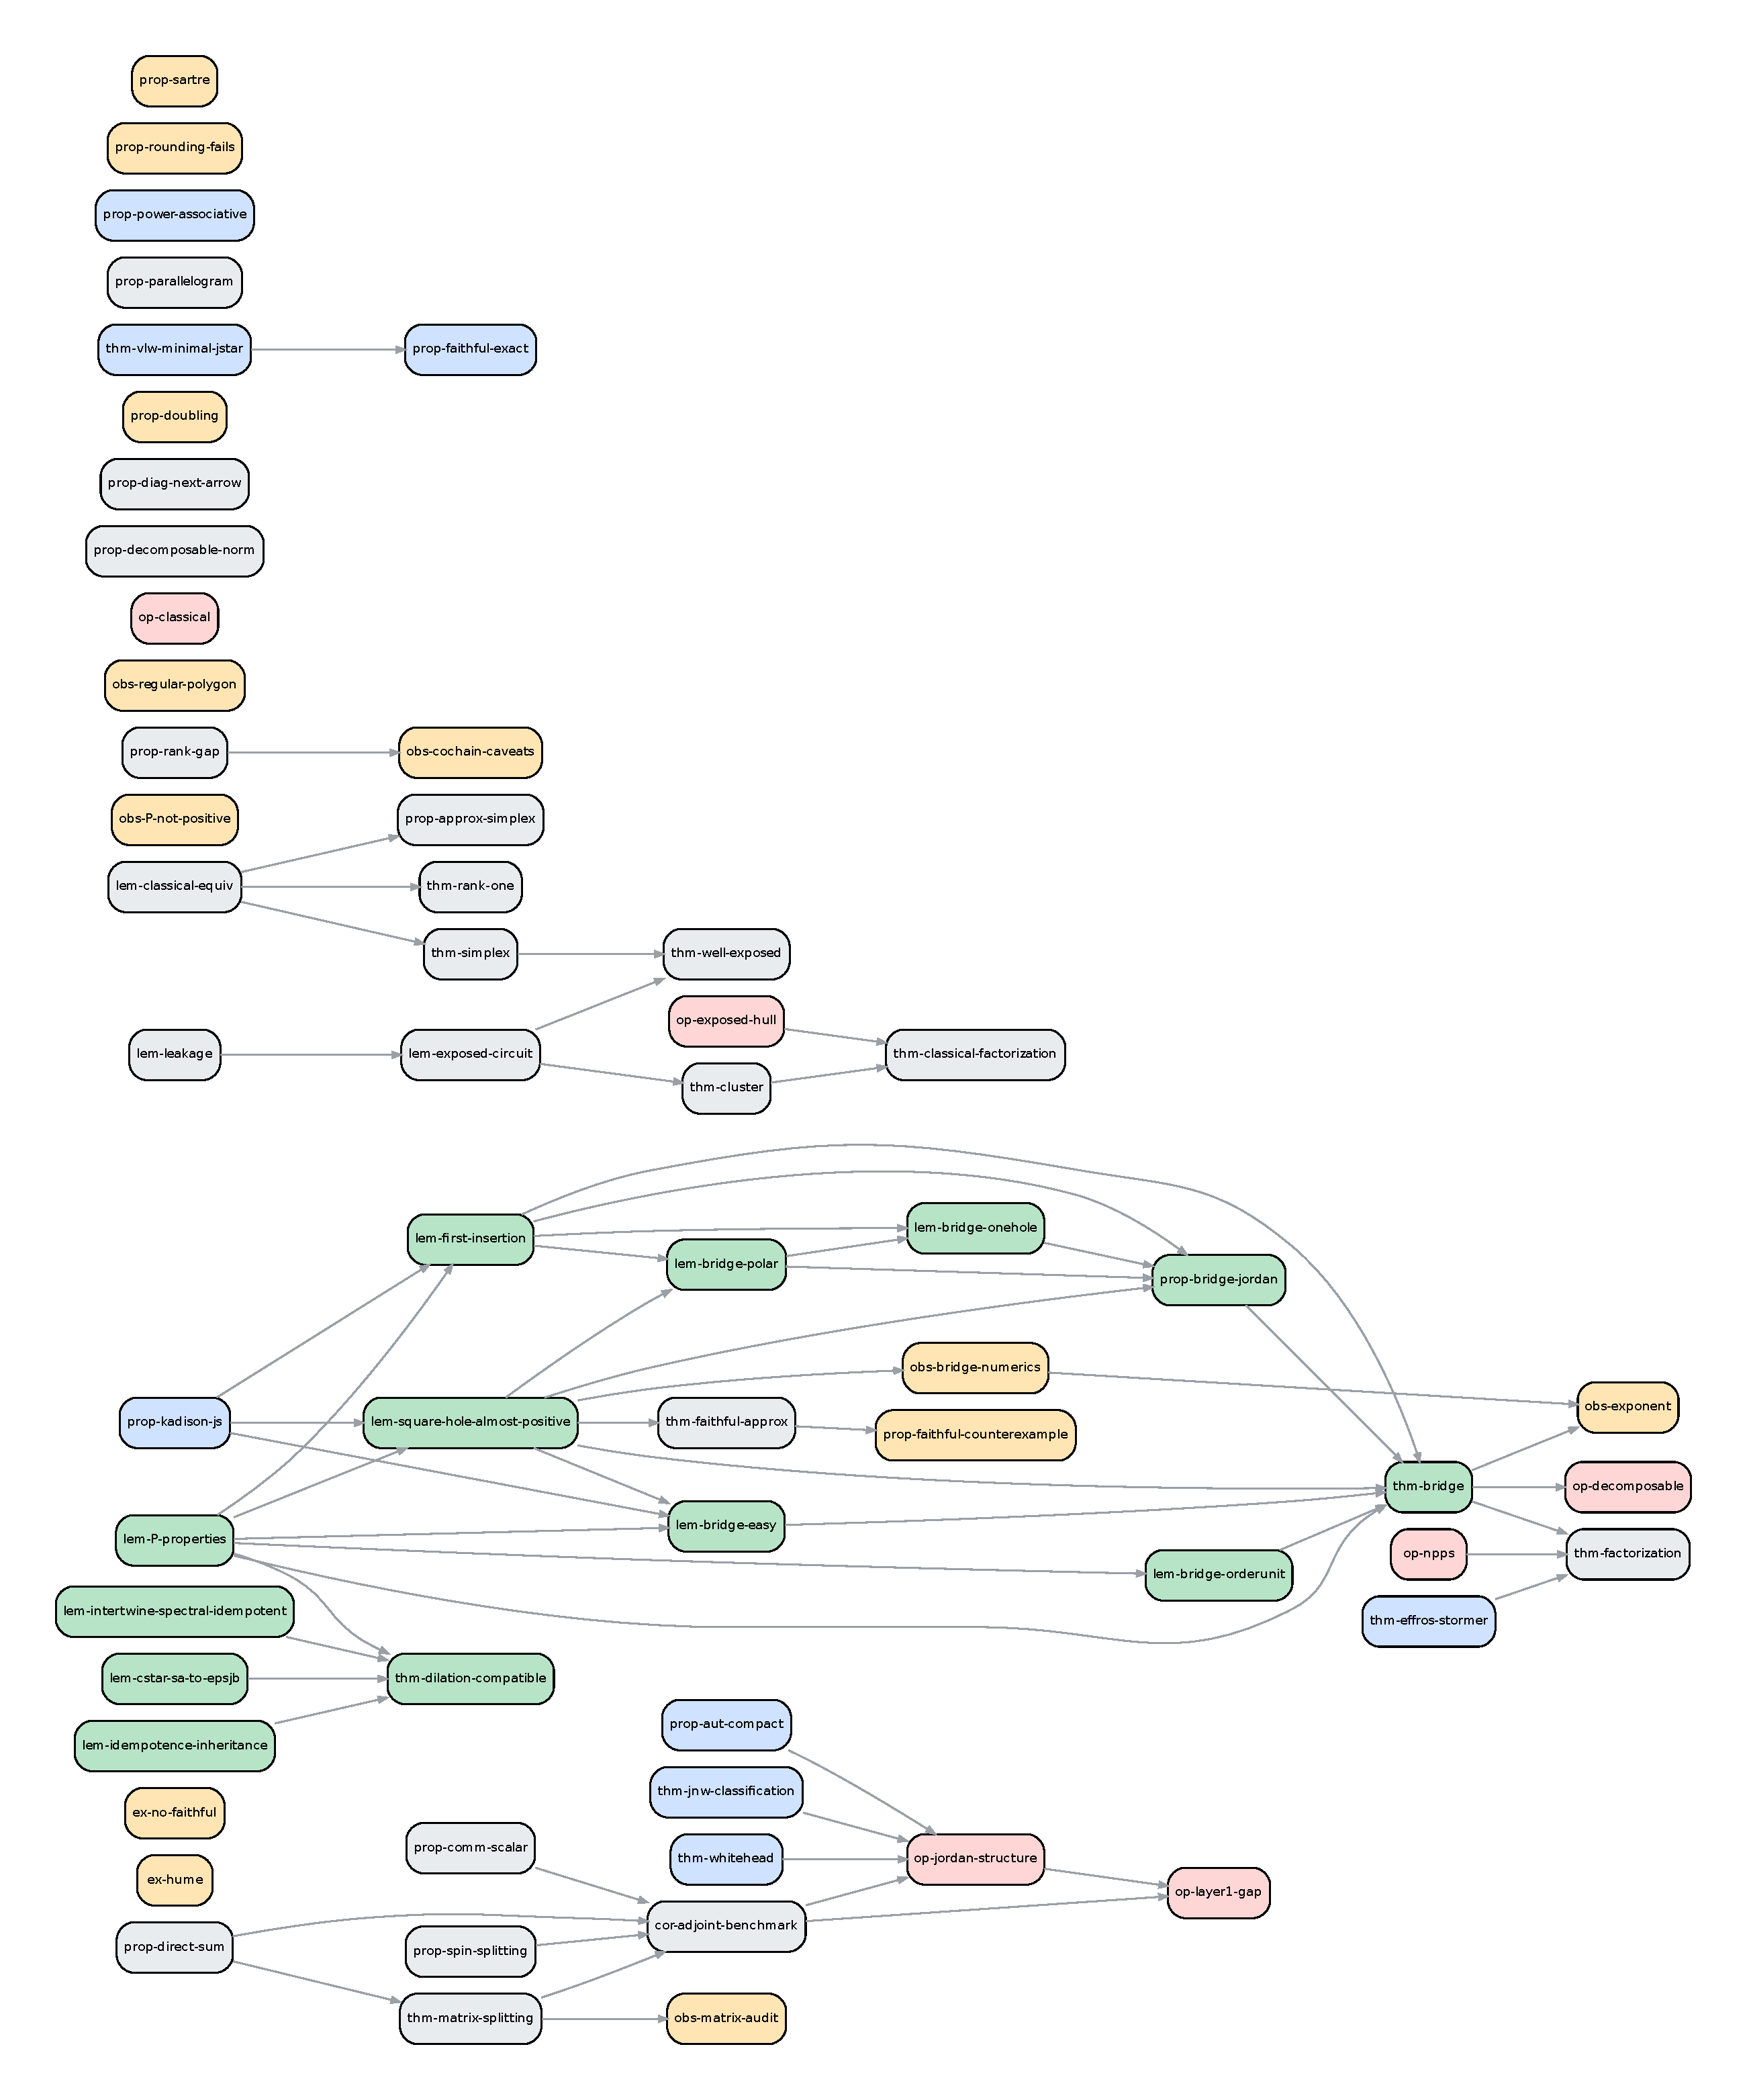
\includegraphics[width=\linewidth,height=0.9\textheight,keepaspectratio]{figures/dag}
\caption{The argument dependency graph, generated from the registry
\texttt{argument/lemmas/} by \texttt{scripts/gen-dag-figure.py}: one node per
result, each edge a dependency. Node colour:
\textcolor{afgreen}{$\blacksquare$~green} = af-validated (machine-checked);
grey = proved in prose but not yet formalised;
blue = cited from the literature;
red = open problem; amber = obstruction / no-go. The PDF is vector graphics:
zoom in a reader to inspect individual node labels.}
\label{fig:dag}
\end{figure}

\subsection{Outlook}

The picture that emerges is uniform. Mere positivity supplies Kadison's
inequality and hence a Jordan, not associative, structure; it supplies one hole
of control, hence the exponent $\sqrt\eta$; and it withholds the dilation that
would supply the second hole, the genuine positivity of $P$, and the
cb-norm-driven dimension-free homotopy. Each open problem is exactly the cost of
one missing piece of complete positivity: the exponent (\Cref{op:decomposable})
is the missing second hole; exact factorization (\Cref{op:npps}) is the missing
positivity of $P$; the abstract structure constant (\Cref{op:layer1-gap}) is
the missing cb-norm/order-unit homotopy, now sharpened by the exact-adjoint
benchmark but still requiring several pre-cohomological and approximate-module
components. None of the three is known to fail. Each has been reduced to
sharply stated remaining packages, not to an unconditional theorem.
